
\documentclass[a4paper,12pt]{article}

\usepackage{url}
\usepackage{graphicx}

\title{PeerSim HOWTO 2: build a topology generator}

\author{Gian Paolo Jesi (jesi@cs.unibo.it)}

\begin{document}

\maketitle

\section{Introduction}

%This section is converted from html, the original can be found under
%\url{http://peersim.sf.net/}. Written by Gian Paolo Jesi.


This tutorial teaches you how to build from scratch a new peersim
( peersim project page: \url{http://sourceforge.net/projects/peersim}
) topology generator. In order to understand this tutorial, the reader
is encouraged to start reading the first peersim tutorial 
(\url{http://peersim. sourceforge.net/peersim_HOWTO.html}) 
to have an idea of the basic concepts that will not be discussed any
further in this document. 

The aim of this tutorial is to be as pratical as possible; the goal
is to give the reader ideas about technical or intermediate level
features of peersim and to encurage him/her to experiment further.
The full source code discussed in this document is available via CVS
at peersim project page in the \emph{peersim.example.hot} class package.


\section{What is a topology?}

The network abstraction in peersim is a (sometimes huge) array of
\emph{Node} structures (interfaces); because of the size of the network
and to overcome scalability problems, usually in large P2P networks
each node knows about the existence of a very small subset of other
nodes (ex: order of log(N) where N is the whole network size). Thus
each node has a short list of other node references, usually called
\char`\"{}neighbors\char`\"{}, build accordingly to some kind of strategy
or rule. 

Thus, we can say that a topology is how nodes are arranged (linked)
together and clearly this depends upon the particular choosen rule.
Examples of topology are the following (not exaustive at all): 

\begin{itemize}
\item random graphs 
\item Watts-Strogatz model graph 
\item star model 
\item ring model 
\item lattice model 
\item ...
\end{itemize}

\subsection{Which rule to choose?}

In this document, we have choosen to code a particular topology generator
to build internet-like tree topologies. The building process is based
on the \emph{preferential attachment} approach. The rule applied is
quite simple and takes into account geometric and network constraints
to better mimic real world network. The preferential attachment choice
can be affected by a parameter ($\alpha$) that amplifies or reduces the
geometric location influence in favor of the path distance. 

The rule strategy is the following: we consider a square unit region
D, then we start with node $x(0)$ choosen at random and we set $W(x(0))
= 0$ (it is the root node). For each i with $i = 1...n-1$ we choose a
new node x(i) in the region $D$ and we connect it to an \textbf{early
inserted} node $x(j)$ that minimize the following formula:

\begin{center}

W(x(j)) + $\alpha$ {*} dist(x(i), x(j)) with 0 $\leq$ j $<$ i
\end{center}

where: 

\begin{itemize}
\item $W(x(j))$ is the distance in terms of hops (the path distance from node
$x(j)$ to the root node); 
\item $dist(...)$ is the usual Euclidean distance; 
\item $\alpha$ is a weight parameter that can minimize or maximize 
the geometric distance influence;
 
\end{itemize}

After having choosen a node $x(j)$, we set $W(x(i)) = W(x(j))+1$ . At
the end we obtain a tree rooted in $x(0)$.

We have extended this model to improve robustness allowing every node
to have exactly d outbound neighbors instead of only one. This means
that at the time of joining the network, each node should have at
least d candidates to be selected as neighbors. To achieve this property,
as a first step we select at random exactly d root nodes and we connect
them together in a ring fashion (a doubly linked list). In this way
each ordinary node has at least d nodes (the d roots) to choose from
in order to select its neighbors; in other words, each node has to
select d nodes that minimize the function above. 

To get further details about this model, we suggest the following
readings:

\begin{enumerate}

\item \char`\"{}Heuristically Optimized Trade-offs: A New Paradigm for Power
Laws in the Internet\char`\"{} 
(\url{http://cgi.di.uoa.gr/~elias/publications/paper-fkp02.pdf} )

\item  \char`\"{}Degree distributions
of the FKP network model\char`\"{} \\
(\url{http://research.microsoft.com/~jchayes/Papers/FKPdgrees.pdf}) 

\item\char`\"{}On Power-Law
Relationships of the Internet Topology\char`\"{}\\ 
(\url{http://www.cs.ucr.edu/~michalis/CAMERA.ps})

\end{enumerate}

The model
should generate a topology that exibits a power-law bound on the in-degree
sequence of nodes; but, as stated in the second previously listed paper,
 this power-law
prediction is not true.

\section{What we need to code}

In order to run this model in peersim we need to write java classes 
extending some peersim tipical interfaces. Very in brief, we need:

\begin{itemize}

\item the protocol class: the protocol itself does nothing because 
we want something that automagically builds this topology model from 
a raw list of unconnected nodes; we are not interested in running any 
piece of code over time (cycles in peersim terminology). This class 
is a sort of structure to collect some needed values such as the node 
space coordinates, the hop distance, the in degree counter and so on. 
The reader can think to this class as \char`\"{}glue code\char`\"{}.
 
\item the initializer class: it extends the \emph{Dynamics} interface and 
deal with all the initialization process. As we'll see further, the 
initializer code itself is very compact because all the building process 
complexity is hidden in a custom made factory pattern class. Please note 
that we don't need explicitly an \emph{Observer} object  because we are 
not interested in observing any behaviour over time; due to that, the code 
to track down informations about the actual generated tree (coordinates 
and indegree distribution) are embeeded into the initializer. 

\end{itemize}

\section{Code writing}

\subsection{Protocol class}

 As we stated so far, the protocol code is minimal:

\footnotesize
\begin{verbatim}
 
 
 import peersim.core.IdleProtocol;
 
 public class InetNodeProtocol extends IdleProtocol {
     // coordinates in space:
     public double x;
     public double y;
     
     public int in_degree;
     public int hops;
     public boolean isroot;
    
     /** Creates a new instance of hotNodeProtocol */
     public InetNodeProtocol(String prefix, Object obj) {
    super(prefix);
         in_degree = 0;
         hops = 0;
         isroot = false;
     }
     
     public Object clone() throws CloneNotSupportedException {
         InetNodeProtocol af = (InetNodeProtocol) super.clone();
         ...
	 return af;
     }
    
     public void nextCycle(peersim.core.Node, int protocolID) {
     }

\end{verbatim}
\normalsize

The \emph{nextCycle()} method is empty, so it's presence is completely 
optional. The class is basically a structure incapsulated in an object.
 
 

\subsection{Initializer class}

 This initializer can be considered as a public interface to the model. 
From the outside (means from the peersim configuration file) only few 
main parameters are needed, such as the \emph{Linkable} enabled protocol, 
the outbound degree and the $\alpha$ parameter. The constructor method 
takes care of collecting these parameters or to set up the corrisponding 
default values The actual structure generation is performed elsewhere.

\footnotesize
\begin{verbatim}
public class InetInitializer implements peersim.dynamics.Dynamics {
     /** 
      * String name of the parameter that defines the protocol to initialize.
     * Parameter read will has the full name
     * <tt>prefix+"."+PAR_PROT</tt>
     */
     public static final String PAR_PROT = "protocol";
 
     /**
      * String name of the parameter about the out degree value.
     */
     public static final String PAR_OUTDEGREE = "d";
     
     /**
      * String name of the parameter used as a weight.
     */
     public static final String PAR_ALFA = "alfa";
     
     /**
      * String name of the parameter used as a maximum x or y coordinate. All the 
      * nodes are on a square region.
     */
     public static final String PAR_MAX_COORD = "max_coord";
    
     ....
     
     /** Creates a new instance of InetInitializer */
     public InetInitializer(String prefix) {
         // super(prefix);
         pid = Configuration.getPid(prefix+"."+PAR_PROT);
         d = Configuration.getInt(prefix+"."+PAR_OUTDEGREE);
         alfa = Configuration.getDouble(prefix+"."+PAR_ALFA);
         graph_filename = "cmplxnet_d"+ d + "_alfa"+alfa+".dat";
         dg_filename = "degree_d"+ d + "_alfa"+alfa+".dat";
         
         maxcoord = Configuration.getDouble(prefix + "." + PAR_MAX_COORD, 1.0);
         if ( !graph_filename.equals("") ) {
             try { graph_fileout = new PrintWriter(new FileWriter(graph_filename)); 
                 System.out.println(prefix +" filename: "+graph_filename +" selected");}
             catch (Exception e) {;}
         }
         if ( !dg_filename.equals("") ) {
             try { dg_fileout = new PrintWriter(new FileWriter(dg_filename)); 
                 System.out.println(prefix +" filename: "+dg_filename +" selected");}
             catch (Exception e) {;}
         }
         
     }
}
\end{verbatim}
\normalsize
     
 The \emph{modify()} method is defined by the \emph{Dynamics} interface;
 it invokes a specialized factory object  that works on top of a 
\emph{OverlayGraph} type object (actual implementation of the \emph{Graph} 
interface).  This object provides the high level abstraction of a graph on 
the simulator overlay network; in this way, it allows the application to 
use many well known graph algorithms and operations (many operations can 
be found in \emph{peersim.graphGraphAlgorithms} class). The operations 
performed on it are reflected on the actual topology (ex: adding an edge).

\footnotesize 
\begin{verbatim}
     public void modify() {
         OverlayGraph ogr = new OverlayGraph(pid);
         InetFactory.InetTree(ogr, CommonRandom.r, pid, maxcoord, d, alfa );
         graphToFile(ogr);
         dgDistribToFile(ogr);
         }
     }
\end{verbatim}
\normalsize

 The other two method invocation in the \emph{modify()} method are 
used to write data on disk. In the first one, for each node $n$ the $x$ 
and $y$ coordinates are collected and then for each neighbor $i$ of node
$n$ the cordinates are written in the following order: 

\footnotesize
\begin{verbatim}
 n.neighbor(i).x n.neighbor(i).y \newline
 n.x n.y \newline
 \newline}
\end{verbatim}
\normalsize 

 The particular line triplet formatting order suits the gluplot needs. 
Please note that the for loop starts from index $d$, not from 0; this means 
that the root node(s) is not directly considered because it has not any 
outbound connections, but only inbound connections. Nevertheless the root 
node(s) are plotted inspecting the nodes that are linked directly to it.

\footnotesize
\begin{verbatim} 
     private void graphToFile(peersim.graph.Graph g) {
         if (graph_fileout != null) { 
             try {
                 for (int i = d ; i < g.size() ; i++ ) {
                     Node current = (Node)g.getNode(i);
                     double x_to = ((InetNodeProtocol)current.getProtocol(pid)).x;
                     double y_to = ((InetNodeProtocol)current.getProtocol(pid)).y;
                     Iterator it = (Iterator)g.getNeighbours(i).iterator();
                     while (it.hasNext()) {
                         int index = ((Integer)it.next()).intValue();
                         Node n = (Node)g.getNode(index);
                         double x_from = ((InetNodeProtocol)n.getProtocol(pid)).x;
                         double y_from = ((InetNodeProtocol)n.getProtocol(pid)).y;
                         
                         graph_fileout.println(x_from+" "+y_from);
                         graph_fileout.println(x_to+" "+y_to);
                         graph_fileout.println("");
                     }
                 }
                 graph_fileout.close();
             }
             catch (Exception e) {;}
         }
     }
\end{verbatim}
\normalsize

 The second data collecting method builds an array of indegree frequencies 
and an array of indegree probability and dumps the second collection to file.

\footnotesize
\begin{verbatim}
private void dgDistribToFile(peersim.graph.Graph g) {
         if (dg_fileout != null) { 
             int size = g.size();
             try {
                 int[] dgfrq = new int[size];
                 double[] dgprob = new double[size];
                 for (int i = 0 ; i < size ; i++) { // do not plot leaves
                     Node n = (Node)g.getNode(i);
                     InetNodeProtocol protocol = (InetNodeProtocol)n.getProtocol(pid);
                     int degree = protocol.in_degree;
                     dgfrq[degree]++;
                 }
                 double sum = 0;
                 for (int i = size-1 ; i > 0 ; i--) {
                     dgprob[i] = (dgfrq[i] + sum)/size;
                     sum += dgfrq[i];
                 }
                 // do not count index 0: 'cos the leafs degree is clearly 0!
                 for (int i = 0 ; i < dgprob.length ; i++ ) {
                     double k = (double)i/size;
                     dg_fileout.println(k+" "+dgprob[i]);
                 }
                 dg_fileout.close();
             }
             catch (Exception e) {e.printStackTrace();
                 System.out.println(e);}
         }   
     }
 }
\end{verbatim}
\normalsize

\section{Factory class}

 This class is the core one. The actual topology initialization is performed 
here. Because of the factory pattern, al the methods in this class are 
static. There is no need of getting parameters from the configuration file, 
because they have been already collected by the initializer class; thus 
the factory is completely hidden.\\
 This implementation is an extention of the peersim standard topology 
factory (\emph{peersim.graph.Graph Factory}).\\

 The only public method is the one that actually builds the topology: 
\emph{InetTree()}; as parameters it gets all the parameters that the 
initializer class has collected. The steps performed are the following:
 
\begin{enumerate} 

\item set the correct values for the $d$ (at least one) roots, including 
coordinates; if there is only one root, its coordinates are centered on 
the square (edge size 1.0 by default), otherwise the coordinates are 
random (as any ordinary node).
 
\item initialize the coordinates and the indegree counter for each 
ordinary node.
 
\item if there are more than one root node, than these root nodes are 
joined together in a ring (connections are non oriented). As an exercise, 
the reader can change this choice implementing something else (ex: putting 
the root nodes in a fully connected topology or a random graph or whatever).
 
\item for each node $n$ other than the root, take exactly $d$ nodes that 
minimizes the formula and connect node n to those d nodes.

\end{enumerate}

The other present methods are all private and can be considered as 
utility methods. Infact their function is quite straightforward and can 
be guessed by the method signature; nevertheless a few comments are 
presented in the following table:

\begin{center}
\begin{tabular}{|l|p{4in}|}
\hline
\emph{getParents()} & get the the current node best d candidates to 
connect to\\
\hline
\emph{hops()} & return the graph distance in terms of hops from the 
root of the node given as a parameter\\
\hline
\emph{minHops()} & return the minimum hop valued node between the 
specified nodes\\
\hline
\emph{distance()} & get the standard Euclideian distance between two nodes\\
\hline
\end{tabular}
\end{center}

\footnotesize
\begin{verbatim}
 
 import hot.HotNodeProtocol;
 import peersim.graph.*;
 import peersim.core.Node;
 import peersim.core.Linkable;
 import peersim.core.Network;
 import peersim.config.Configuration;
 import java.util.Random;
 import java.util.ArrayList;
 import java.util.Arrays;
 
 public class InetFactory extends peersim.graph.GraphFactory {
     
     private static final String DEBUG_STRING = "inet.InetFactory: ";
    
     public InetFactory() {
         super();
     }
     
     public static Graph InetTree(Graph g, Random rnd, int pid, double maxcoord,
     int outdegree, double alfa) {
         int size = g.size(); // size of the network
         System.out.println(DEBUG_STRING+"size: "+size+" outdegree: "+outdegree);
   
         // build outdegree roots
         System.out.println(DEBUG_STRING+"Generating "+outdegree+" root(s), 
	 means out degree "+outdegree+"...");
         for(int i = 0 ; i < outdegree ; ++i) {
             Node n = (Node)g.getNode(i);
             HotNodeProtocol prot = (HotNodeProtocol)n.getProtocol(pid);
             prot.isroot = true;
             prot.hops = 0;
             prot.in_degree = 0;
             if (outdegree == 1 ) {
                 prot.x = maxcoord/2;
                 prot.y = maxcoord/2;
             }
             else { // more than one root
                 if (rnd.nextBoolean() ) {
                     prot.x = maxcoord/2 + (rnd.nextDouble() * 0.1);
                 }
                 else {
                     prot.x = maxcoord/2 - (rnd.nextDouble() * 0.1);
                 }
                 if (rnd.nextBoolean() ) {
                     prot.y = maxcoord/2 + (rnd.nextDouble() * 0.1);
                 }
                 else {
                     prot.y = maxcoord/2 - (rnd.nextDouble() * 0.1);
                 }
                 System.out.println("root coord: "+prot.x+" "+prot.y);
             }
         }
         
         // Set coordinates x,y and set indegree 0
         System.out.println(DEBUG_STRING+"Generating random cordinates for nodes...");
         for (int i = outdegree ; i < size ; i++) {
             Node n = (Node)g.getNode(i);
             HotNodeProtocol prot = (HotNodeProtocol)n.getProtocol(pid);
             if (maxcoord == 1.0) {
                 prot.x = rnd.nextDouble();
                 prot.y = rnd.nextDouble();
             }
             else {
                 prot.x = rnd.nextInt((int)maxcoord);
                 prot.y = rnd.nextInt((int)maxcoord);
             }
             prot.in_degree = 0;
         }
       
         // Connect the roots in a ring if needed (thus, if there are more than 1
         // root nodes.
         if (outdegree > 1) {
             System.out.println(DEBUG_STRING+"Putting roots in a ring...");
             for (int i = 0 ; i < outdegree ; i++) {
                 Node n = (Node)g.getNode(i);
                 ((HotNodeProtocol)n.getProtocol(pid)).in_degree++;
                 n = (Node)g.getNode(i+1);
                 ((HotNodeProtocol)n.getProtocol(pid)).in_degree++;
                 
                 g.setEdge(i, i+1);
                 g.setEdge(i+1, i);
             }
             Node n = (Node)g.getNode(0);
             ((HotNodeProtocol)n.getProtocol(pid)).in_degree++;
             n = (Node)g.getNode(outdegree);
             ((HotNodeProtocol)n.getProtocol(pid)).in_degree++;
             g.setEdge(0, outdegree);
             g.setEdge(outdegree, 0);
         }
         
         // for all the nodes other than root(s), connect them!
         for (int i = outdegree ; i < size ; ++i ) {
             Node n = (Node)g.getNode(i);
             InetNodeProtocol prot = (InetNodeProtocol)n.getProtocol(pid);
             
             prot.isroot = false;
             
             // look for a siutable parent node between those allready part of the
             // overlay topology: alias FIND THE MINIMUM!
             Node candidate = null;
             int candidate_index = 0;
             double min = Double.POSITIVE_INFINITY;
             if (outdegree > 1) {
                     int candidates[] = getParents(g, pid, i, outdegree, alfa);
                     for (int s = 0 ; s < candidates.length ; s++) {
                         g.setEdge(i, candidates[s]);
                         System.out.print(i+", ");
                     }
                     prot.hops = minHop(g, candidates, pid) + 1;
             }
             else { // degree 1:
                 for (int j = 0 ; j < i ; j++) {
                     Node parent = (Node)g.getNode(j);
                     InetNodeProtocol prot_parent = (InetNodeProtocol)parent.getProtocol(pid);
                           
                     double value = hops(parent, pid) + 
                         (alfa * distance(n, parent, pid));
                     if (value < min) {
                         candidate = parent; // best parent node to connect to
                         min = value;
                         candidate_index = j;
                     }   
                 }
                 prot.hops = ((InetNodeProtocol)candidate.getProtocol(pid)).hops + 1; 
                 g.setEdge(i, candidate_index);
                 ((HotNodeProtocol)candidate.getProtocol(pid)).in_degree++;
             }
             
         }
         System.out.println(DEBUG_STRING+"Graph generation finished!");
         return g;
     }
     
     private static int[] getParents(Graph g, int pid, int cur_node_index,
     int how_many, double alfa) {
         int result[] = new int[how_many];
         ArrayList net_copy = new ArrayList(cur_node_index);
         // fill up the sub net copy:
         for (int j = 0 ; j < cur_node_index ; j++) {
             net_copy.add(j, (Node)g.getNode(j));
         }
         
         // it needs exactly how_many minimums!
         for (int k = 0 ; k < how_many ; k++) {
             int candidate_index = 0;
             double min = Double.POSITIVE_INFINITY;
             // for all the elements in the copy...
             for (int j = 0 ; j < net_copy.size() ; j++) {
                 Node parent = (Node)net_copy.get(j);
                 HotNodeProtocol prot_parent = (HotNodeProtocol)parent.getProtocol(pid);
                 double value = hops(parent, pid) + (alfa * 
                     distance((Node)g.getNode(cur_node_index), parent, pid));
             
                 if (value < min) {
                     min = value;
                     candidate_index = j;
                 }
             }
             result[k] = candidate_index;        // collect the parent node
             net_copy.remove(candidate_index); // delete the min from the net copy 
         }
         return result;
     }
     
 
     private static int hops(Node node, int pid) {
         return ((HotNodeProtocol)node.getProtocol(pid)).hops;
     }
     
     private static int minHop(Graph g, int[] indexes, int pid) {
         int min = Integer.MAX_VALUE; 
         for (int s = 0 ; s < indexes.length ; s++) {
             Node parent = (Node)g.getNode(indexes[s]);
             int value = ((HotNodeProtocol)parent.getProtocol(pid)).hops;
             if (value < min) {
                 min = value;
             }   
         }
         return min;
     }
      
     private static double distance(Node new_node, Node old_node, int pid) {
         // Eucleidian distance code...
     } 
 }
\end{verbatim}
\normalsize

\section{Experiments}

 In order to make the model run, a proper peersim configuration file is 
needed. The one presented in the following lines may suits the reader needs:

\footnotesize
\begin{verbatim}
 # Complex Network file:
 random.seed 1234567890
 simulation.cycles 1
 
 overlay.size 10000
 overlay.maxSize 10000
 
 protocol.0 hot.InetNodeProtocol
 #protocol.0.maxcoord 1000
 
 init.0 hot.InetInitializer
 init.0.alfa 20
 init.0.protocol 0
 init.0.d 1
\end{verbatim}
\normalsize

 It produces a 10000 node overlay network with the parameters listed in 
the \texttt{init.0} section.\\
 The figures in the table shows the produced topology and highlights the 
parameter $\alpha$ importance. Infact it affects the clustering behaviour of 
the system and it is tightly correlated to the size of the network. If 
$\alpha$ il lower than $\sqrt{netsize}$, the topology becomes more and more 
clusterized (as show in the first two figures); with extremely low $\alpha$, 
the topology becomes a star. On the other end, if $\alpha$ is grater than 
$\sqrt{netsize}$, the topology tends to be random and not clusterized at all 
(the second row of images). For deeper details, please consult the previously
listed papers.\\

All the images has been produced using only one root node and only 
one outbound connection per node. Using two or more outbound connection 
per node leads to a massively crowded plot, so it's not a very nice picture 
to plot!\\

\begin{figure}
\begin{center}
\includegraphics[scale=0.6]{pic_alfa01.eps}
\end{center}
\caption{Topology with $\alpha$ 0.1\label{t01figure}}
\end{figure}



The degree distribution related to the generated star topology 
(Figure\ref{t01figure}) is not 
shown (it's simply a straight line).
Clearly the plots show that there is not any evidence about in-degree 
power-law distribution; only in the case of $\alpha = 4$, the corrisponding 
plot exibits a power-law like behaviour at least for a subset of the nodes, 
but this is very different from what first listed paper was talking about.

\begin{figure}
\begin{center}
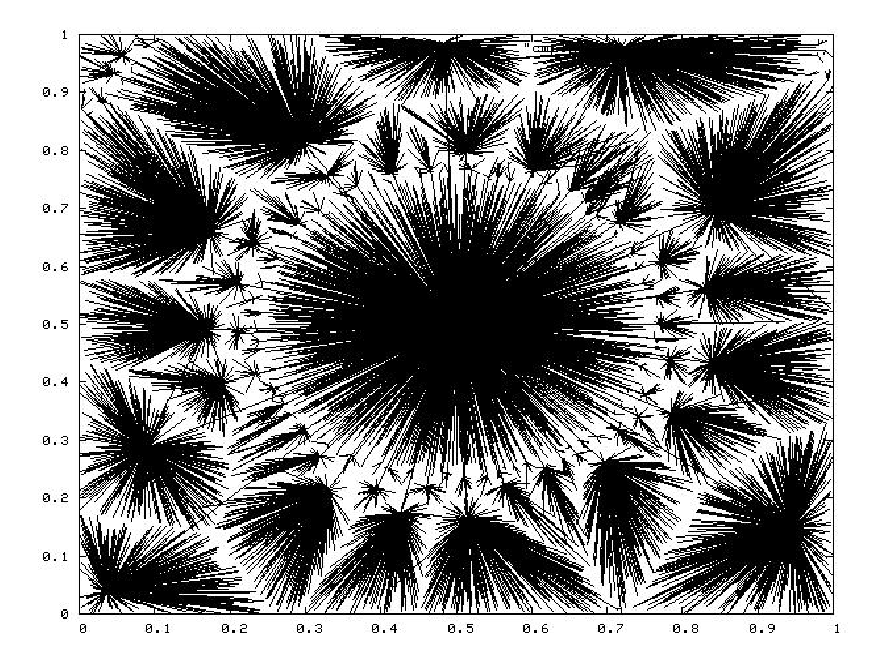
\includegraphics[scale=0.6]{pic_alfa4.eps}
\end{center}
\caption{Topology with $\alpha$ 4\label{t4figure}}
\end{figure}

\begin{figure}
\begin{center}
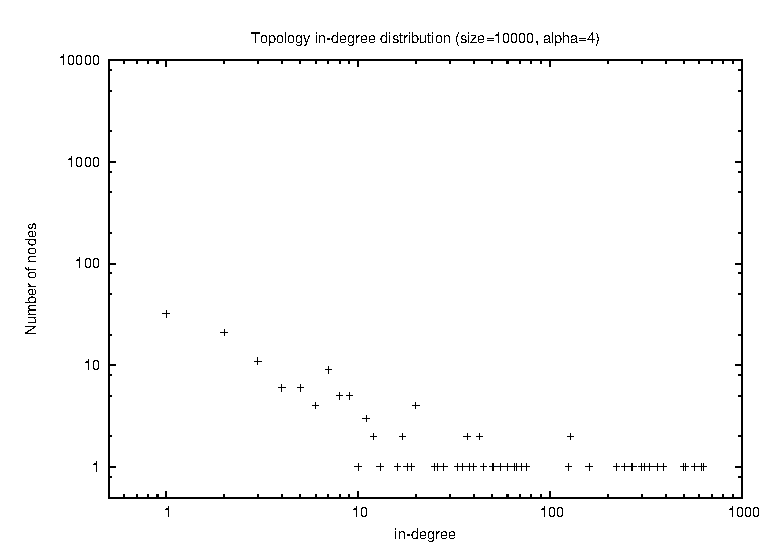
\includegraphics[scale=0.6]{picdegree_alfa4.eps}
\end{center}
\caption{Indegree distribution with $\alpha$ 4 \label{d4figure}}
\end{figure}

\begin{figure}
\begin{center}
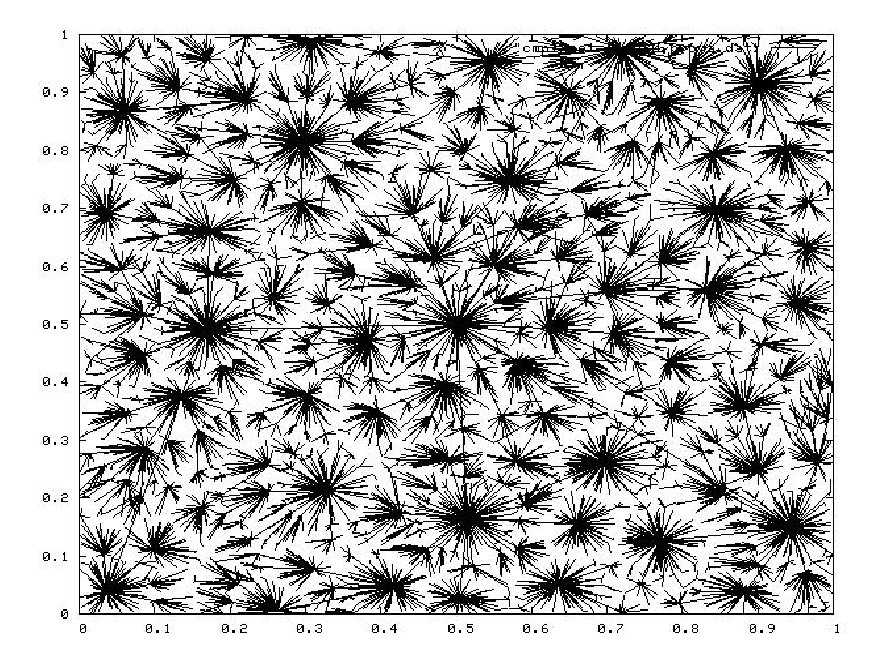
\includegraphics[scale=0.6]{pic_alfa20.eps}
\end{center}
\caption{Topology with $\alpha$ 20\label{t20figure}}
\end{figure}

\begin{figure}
\begin{center}
\includegraphics[scale=0.6]{picdegree_alfa20.eps}
\end{center}
\caption{Indegree distribution with $\alpha$ 20 \label{d20figure}}
\end{figure}

\begin{figure}
\begin{center}
\includegraphics[scale=0.6]{pic_alfa100.eps}
\end{center}
\caption{Topology with $\alpha$ 100\label{t100figure}}
\end{figure}

\begin{figure}
\begin{center}
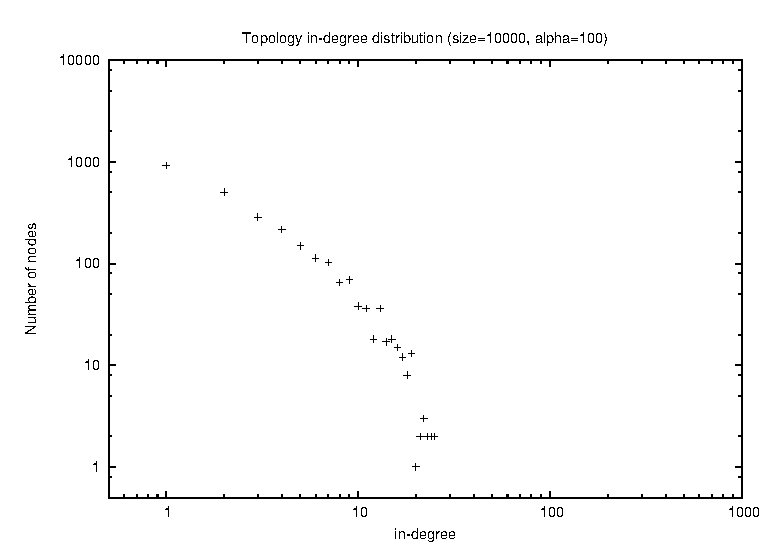
\includegraphics[scale=0.6]{picdegree_alfa100.eps}
\end{center}
\caption{Indegree distribution with $\alpha$ 100\label{d100figure}}
\end{figure}

\begin{figure}
\begin{center}
\includegraphics[scale=0.6]{pic_alfa2000.eps}
\end{center}
\caption{Topology with $\alpha$ 2000\label{t2000figure}}
\end{figure}

\begin{figure}
\begin{center}
\includegraphics[scale=0.6]{picdegree_alfa2000.eps}
\end{center}
\caption{Indegree distribution with $\alpha$ 2000\label{d2000figure}}
\end{figure}

\end{document}
